\section{Results}
%-------------------------------------------------------------------------------------------




%-------------------------------------------------------------------------------------------

\subsection{Static environment}

%-------------------------------------------------------------------------------------------
% Maze 1

The paths taken by the algorithms when the environment was static and maze 1 was used, can be seen in Fig.\:\ref{fig:static_path_maze_1}. Fig.\:\ref{fig:a_star_static_path_maze_1} shows the path taken by A*, Dijkstra is shown in Fig.\:\ref{fig:dijkstra_static_path_maze_1}, and finally D* lite is shown in Fig.\:\ref{fig:d_star_static_path_maze_1}.

\begin{figure}
	\centering
    \begin{subfigure}[t]{0.32\columnwidth}
		\centering
		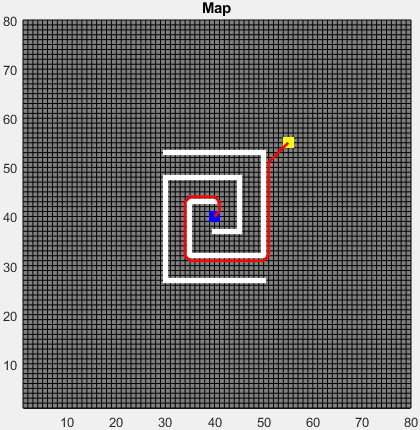
\includegraphics[width=\textwidth]{images/a_star_static_maze_1.png}
		\caption{Path taken by A* assuming static environment in maze 1.}
        \label{fig:a_star_static_path_maze_1}
	\end{subfigure}
    \hfill
	\begin{subfigure}[t]{0.32\columnwidth}
		\centering
		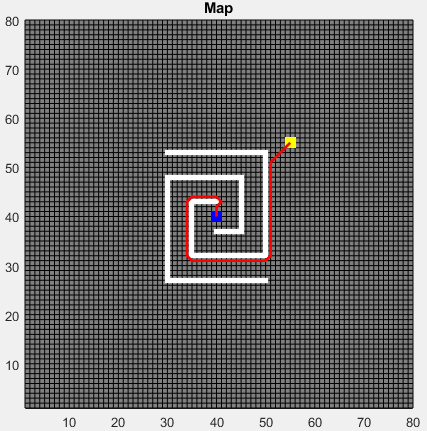
\includegraphics[width=\textwidth]{images/dijkstra_static_maze_1.png}
		\caption{Path taken by Dijkstra assuming static environment in maze 1.}
        \label{fig:dijkstra_static_path_maze_1}
	\end{subfigure}
    \hfill
    \begin{subfigure}[t]{0.32\columnwidth}
		\centering
		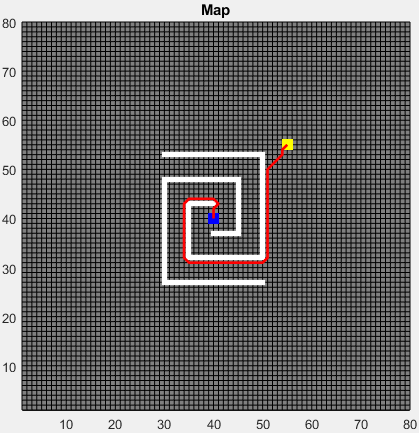
\includegraphics[width=\textwidth]{images/d_star_lite_static_maze_1.png}
		\caption{Path taken by D* lite assuming static environment in maze 1.}
        \label{fig:d_star_static_path_maze_1}
	\end{subfigure}
	\caption{Paths taken by all algorithms assuming static environment in maze 1.}
    \label{fig:static_path_maze_1}
\end{figure}

The evaluation measurements of all algorithms for static environment in maze 1 can be seen in Table.\:\ref{tab:metric_static_maze_1}.

\begin{table}
    \centering
    \begin{tabular}{c|c|c|c}
        Algorithm   & Pushes    & Pops      & Execution time (s)    \\ \hline
        A*          & $549$     & $503$     & $1.0489$              \\
        Dijkstra    & $3373$    & $3078$    & $37.2224$             \\
        D* lite     & $2805$    & $2524$    & $27.9366$
    \end{tabular}
    \caption{Evaluation measurements of all algorithms assuming static environment in maze 1.}
    \label{tab:metric_static_maze_1}
\end{table}

%-------------------------------------------------------------------------------------------
% Maze 2

Fig.\:\ref{fig:static_path_maze_2} presents the paths taken in static environment for maze 2. Fig.\:\ref{fig:a_star_static_path_maze_2} shows the path taken by A*, Dijkstra is shown in Fig.\:\ref{fig:dijkstra_static_path_maze_2}, and finally D* lite is shown in Fig.\:\ref{fig:d_star_static_path_maze_2}.

\begin{figure}
	\centering
    \begin{subfigure}[t]{0.32\columnwidth}
		\centering
		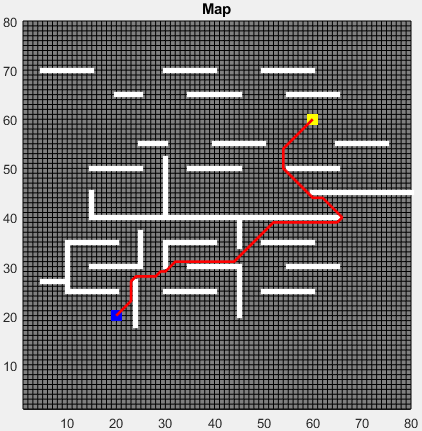
\includegraphics[width=\textwidth]{images/a_star_static_maze_2.png}
		\caption{Path taken by A* assuming static environment in maze 2.}
        \label{fig:a_star_static_path_maze_2}
	\end{subfigure}
    \hfill
	\begin{subfigure}[t]{0.32\columnwidth}
		\centering
		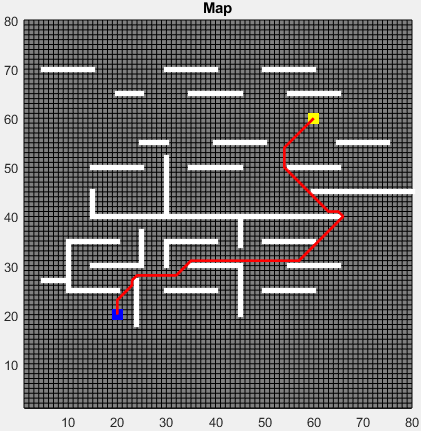
\includegraphics[width=\textwidth]{images/dijkstra_static_maze_2.png}
		\caption{Path taken by Dijkstra assuming static environment in maze 2.}
        \label{fig:dijkstra_static_path_maze_2}
	\end{subfigure}
    \hfill
    \begin{subfigure}[t]{0.32\columnwidth}
		\centering
		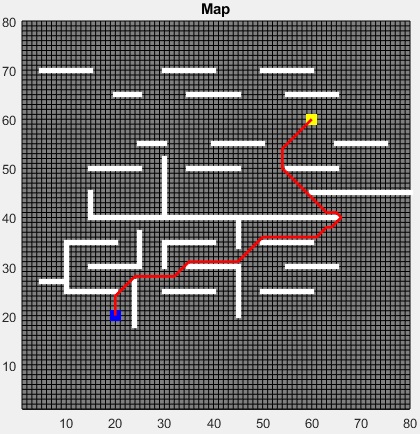
\includegraphics[width=\textwidth]{images/d_star_lite_static_maze_2.png}
		\caption{Path taken by D* lite assuming static environment in maze 2.}
        \label{fig:d_star_static_path_maze_2}
	\end{subfigure}
	\caption{Paths taken by all algorithms assuming static environment in maze 2.}
    \label{fig:static_path_maze_2}
\end{figure}

The evaluation measurements of all algorithms for static environment in maze 2 can be seen in Table.\:\ref{tab:metric_static_maze_2}.

\begin{table}
    \centering
    \begin{tabular}{c|c|c|c}
        Algorithm   & Pushes    & Pops      & Execution time (s)    \\ \hline
        A*          & $2649$    & $2440$    & $20.1303$             \\
        Dijkstra    & $5380$    & $5319$    & $38.893$              \\
        D* lite     & $2686$    & $2407$    & $19.5628$
    \end{tabular}
    \caption{Evaluation measurements of all algorithms assuming static environment in maze 2.}
    \label{tab:metric_static_maze_2}
\end{table}

%-------------------------------------------------------------------------------------------
% Maze 3

The paths taken through maze 3 by all the algorithms when the environment was static is shown in Fig.\:\ref{fig:static_path_maze_3}. Fig.\:\ref{fig:a_star_static_path_maze_3} shows the path taken by A*, Dijkstra is shown in Fig.\:\ref{fig:dijkstra_static_path_maze_3}, and finally D* lite is shown in Fig.\:\ref{fig:d_star_static_path_maze_3}.

\begin{figure}
	\centering
    \begin{subfigure}[t]{0.32\columnwidth}
		\centering
		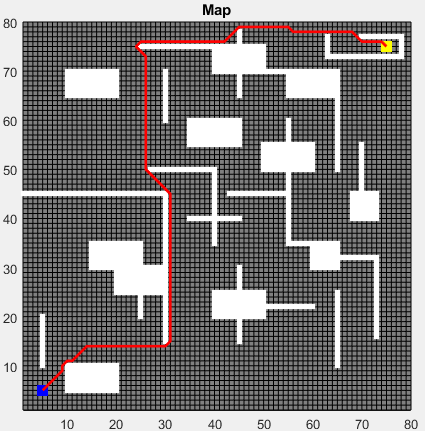
\includegraphics[width=\textwidth]{images/a_star_static_maze_3.png}
		\caption{Path taken by A* assuming static environment in maze 3.}
        \label{fig:a_star_static_path_maze_3}
	\end{subfigure}
    \hfill
	\begin{subfigure}[t]{0.32\columnwidth}
		\centering
		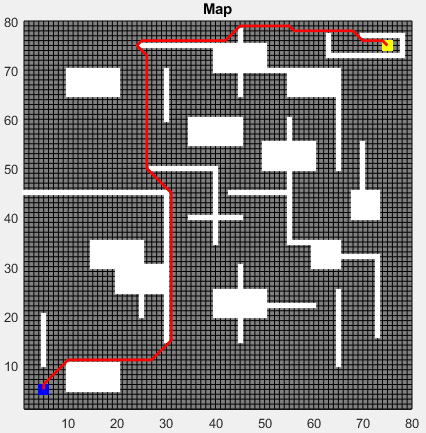
\includegraphics[width=\textwidth]{images/dijkstra_static_maze_3.png}
		\caption{Path taken by Dijkstra assuming static environment in maze 3.}
        \label{fig:dijkstra_static_path_maze_3}
	\end{subfigure}
    \hfill
    \begin{subfigure}[t]{0.32\columnwidth}
		\centering
		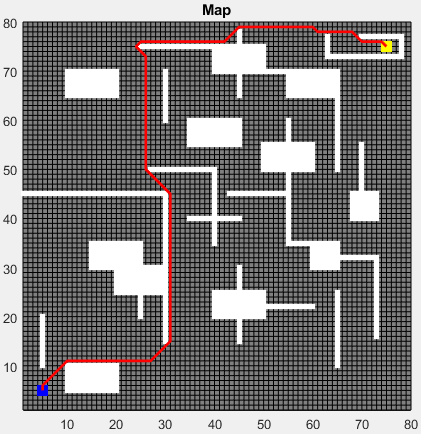
\includegraphics[width=\textwidth]{images/d_star_lite_static_maze_3.png}
		\caption{Path taken by D* lite assuming static environment in maze 3.}
        \label{fig:d_star_static_path_maze_3}
	\end{subfigure}
	\caption{Paths taken by all algorithms assuming static environment in maze 3.}
    \label{fig:static_path_maze_3}
\end{figure}

The evaluation measurements of all algorithms for static environment in maze 3 can be seen in Table.\:\ref{tab:metric_static_maze_3}.

\begin{table}
    \centering
    \begin{tabular}{c|c|c|c}
        Algorithm   & Pushes    & Pops      & Execution time (s)    \\ \hline
        A*          & $4953$    & $4873$    & $37.4206$             \\
        Dijkstra    & $5436$    & $5433$    & $30.7629$             \\
        D* lite     & $3348$    & $3181$    & $20.836$
    \end{tabular}
    \caption{Evaluation measurements of all algorithms assuming static environment in maze 3.}
    \label{tab:metric_static_maze_3}
\end{table}

%-------------------------------------------------------------------------------------------




%-------------------------------------------------------------------------------------------

\subsection{Dynamic environment}

%-------------------------------------------------------------------------------------------
% Maze 1

The paths taken by the algorithms when the environment was dynamic and maze 1 was used, can be seen in Fig.\:\ref{fig:dynamic_path_maze_1}. Fig.\:\ref{fig:a_star_dynamic_path_maze_1} shows the path taken by A*, Dijkstra is shown in Fig.\:\ref{fig:dijkstra_dynamic_path_maze_1}, and finally D* lite is shown in Fig.\:\ref{fig:d_star_dynamic_path_maze_1}.

\begin{figure}
	\centering
    \begin{subfigure}[t]{0.32\columnwidth}
		\centering
		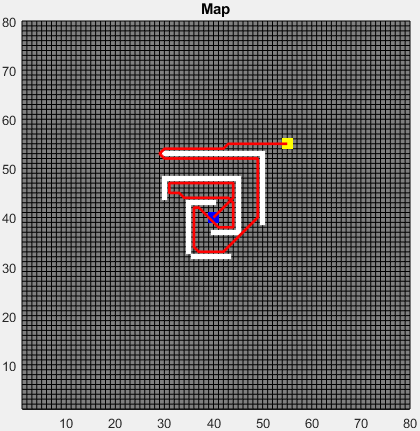
\includegraphics[width=\textwidth]{images/a_star_dynamic_maze_1.png}
		\caption{Path taken by A* assuming dynamic environment in maze 1.}
        \label{fig:a_star_dynamic_path_maze_1}
	\end{subfigure}
    \hfill
	\begin{subfigure}[t]{0.32\columnwidth}
		\centering
		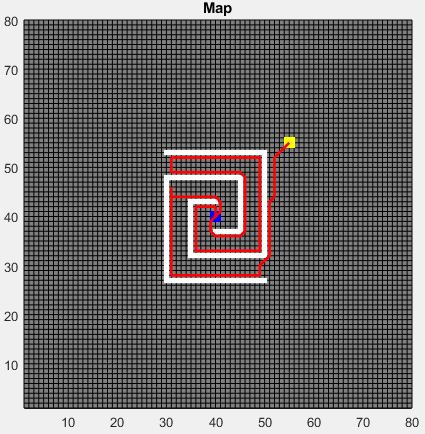
\includegraphics[width=\textwidth]{images/dijkstra_dynamic_maze_1.png}
		\caption{Path taken by Dijkstra assuming dynamic environment in maze 1.}
        \label{fig:dijkstra_dynamic_path_maze_1}
	\end{subfigure}
    \hfill
    \begin{subfigure}[t]{0.32\columnwidth}
		\centering
		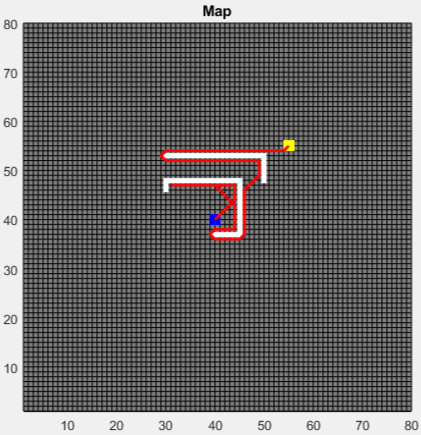
\includegraphics[width=\textwidth]{images/d_star_lite_dynamic_maze_1.png}
		\caption{Path taken by D* lite assuming dynamic environment in maze 1.}
        \label{fig:d_star_dynamic_path_maze_1}
	\end{subfigure}
	\caption{Paths taken by all algorithms assuming dynamic environment in maze 1.}
    \label{fig:dynamic_path_maze_1}
\end{figure}

The evaluation measurements of all algorithms for dynamic environment in maze 1 can be seen in Table.\:\ref{tab:metric_dynamic_maze_1}.

\begin{table}
    \centering
    \begin{tabular}{c|c|c|c}
        Algorithm   & Pushes    & Pops      & Execution time (s)    \\ \hline
        A*          & $2779$    & $1713$    & $2.7427$              \\
        Dijkstra    & $3683$    & $2468$    & $15.7218$             \\
        D* lite     & $1206$    & $1031$    & $7.9151$
    \end{tabular}
    \caption{Evaluation measurements of all algorithms assuming dynamic environment in maze 1.}
    \label{tab:metric_dynamic_maze_1}
\end{table}

%-------------------------------------------------------------------------------------------
% Maze 2

The paths taken through maze 2 when the environment was dynamic, can be seen in Fig.\:\ref{fig:dynamic_path_maze_2}. Fig.\:\ref{fig:a_star_dynamic_path_maze_2} shows the path taken by A*, Dijkstra is shown in Fig.\:\ref{fig:dijkstra_dynamic_path_maze_2}, and finally D* lite is shown in Fig.\:\ref{fig:d_star_dynamic_path_maze_2}.

\begin{figure}
	\centering
    \begin{subfigure}[t]{0.32\columnwidth}
		\centering
		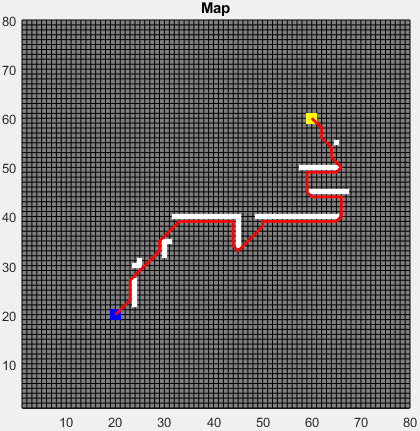
\includegraphics[width=\textwidth]{images/a_star_dynamic_maze_2.png}
		\caption{Path taken by A* assuming dynamic environment in maze 2.}
        \label{fig:a_star_dynamic_path_maze_2}
	\end{subfigure}
    \hfill
	\begin{subfigure}[t]{0.32\columnwidth}
		\centering
		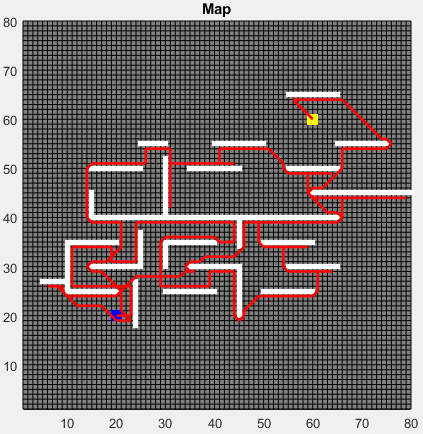
\includegraphics[width=\textwidth]{images/dijkstra_dynamic_maze_2.png}
		\caption{Path taken by Dijkstra assuming dynamic environment in maze 2.}
        \label{fig:dijkstra_dynamic_path_maze_2}
	\end{subfigure}
    \hfill
    \begin{subfigure}[t]{0.32\columnwidth}
		\centering
		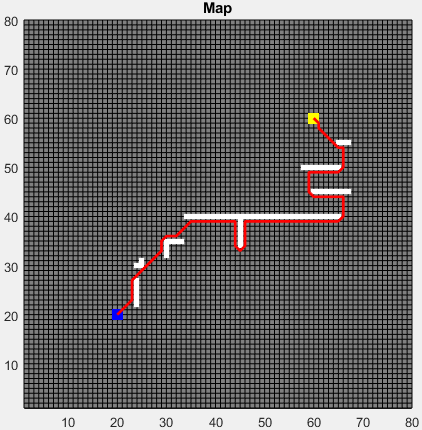
\includegraphics[width=\textwidth]{images/d_star_lite_dynamic_maze_2.png}
		\caption{Path taken by D* lite assuming dynamic environment in maze 2.}
        \label{fig:d_star_dynamic_path_maze_2}
	\end{subfigure}
	\caption{Paths taken by all algorithms assuming dynamic environment in maze 2.}
    \label{fig:dynamic_path_maze_2}
\end{figure}

The evaluation measurements of all algorithms for dynamic environment in maze 2 can be seen in Table.\:\ref{tab:metric_dynamic_maze_2}.

\begin{table}
    \centering
    \begin{tabular}{c|c|c|c}
        Algorithm   & Pushes    & Pops      & Execution time (s)    \\ \hline
        A*          & $693$     & $229$     & $0.27295$             \\
        Dijkstra    & $11858$   & $8532$    & $41.4283$             \\
        D* lite     & $1170$    & $904$     & $11.811$
    \end{tabular}
    \caption{Evaluation measurements of all algorithms assuming dynamic environment in maze 2.}
    \label{tab:metric_dynamic_maze_2}
\end{table}

%-------------------------------------------------------------------------------------------
% Maze 3

Fig.\:\ref{fig:dynamic_path_maze_3} presents the paths taken through maze 3 by all algorithms when the environment was dynamic. Fig.\:\ref{fig:a_star_dynamic_path_maze_3} shows the path taken by A*, Dijkstra is shown in Fig.\:\ref{fig:dijkstra_dynamic_path_maze_3}, and finally D* lite is shown in Fig.\:\ref{fig:d_star_dynamic_path_maze_3}.

\begin{figure}
	\centering
    \begin{subfigure}[t]{0.32\columnwidth}
		\centering
		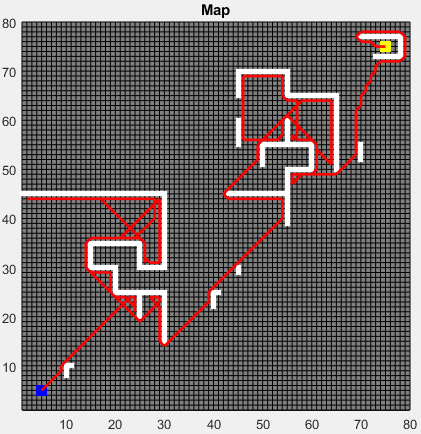
\includegraphics[width=\textwidth]{images/a_star_dynamic_maze_3.png}
		\caption{Path taken by A* assuming dynamic environment in maze 3.}
        \label{fig:a_star_dynamic_path_maze_3}
	\end{subfigure}
    \hfill
	\begin{subfigure}[t]{0.32\columnwidth}
		\centering
		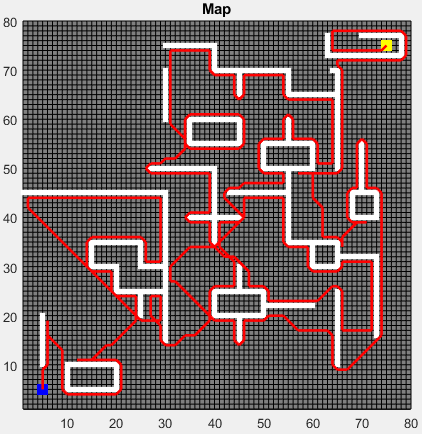
\includegraphics[width=\textwidth]{images/dijkstra_dynamic_maze_3.png}
		\caption{Path taken by Dijkstra assuming dynamic environment in maze 3.}
        \label{fig:dijkstra_dynamic_path_maze_3}
	\end{subfigure}
    \hfill
    \begin{subfigure}[t]{0.32\columnwidth}
		\centering
		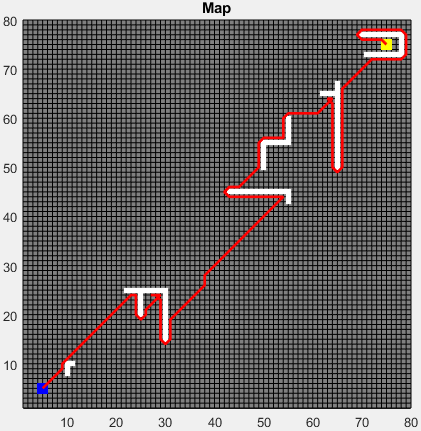
\includegraphics[width=\textwidth]{images/d_star_lite_dynamic_maze_3.png}
		\caption{Path taken by D* lite assuming dynamic environment in maze 3.}
        \label{fig:d_star_dynamic_path_maze_3}
	\end{subfigure}
	\caption{Paths taken by all algorithms assuming dynamic environment in maze 3.}
    \label{fig:dynamic_path_maze_3}
\end{figure}

The evaluation measurements of all algorithms for dynamic environment in maze 3 can be seen in Table.\:\ref{tab:metric_dynamic_maze_3}.

\begin{table}
    \centering
    \begin{tabular}{c|c|c|c}
        Algorithm   & Pushes    & Pops      & Execution time (s)    \\ \hline
        A*          & $7210$    & $4356$    & $7.5347$              \\
        Dijkstra    & $14634$   & $9867$    & $31.382$              \\
        D* lite     & $2593$    & $2155$    & $47.4293$
    \end{tabular}
    \caption{Evaluation measurements of all algorithms assuming dynamic environment in maze 3.}
    \label{tab:metric_dynamic_maze_3}
\end{table}

%-------------------------------------------------------------------------------------------